%-briefly recaps the project purposes and goals,
\documentclass[onecolumn, draftclsnofoot,10pt, compsoc]{IEEEtran}
\usepackage{graphicx}
\usepackage{url}
\usepackage{setspace}
\usepackage{cite}
\usepackage{tabularx}
\usepackage{listings}
\usepackage{longtable}
\usepackage{minted}
\usepackage{float}

\usepackage{geometry}
\geometry{textheight=9.5in, textwidth=7in}



% 1. Fill in these details
\def \CapstoneTeamName{		Auction Hunter}
\def \CapstoneTeamNumber{		4}
\def \GroupMemberOne{			Alexander Hull}
\def \GroupMemberTwo{			Alexander Jacobson}
\def \GroupMemberThree{			Yufei Zeng}
\def \CapstoneProjectName{		Auction Hunter}
\def \CapstoneSponsorCompany{	}
\def \CapstoneSponsorPerson{		Ryan Kalb}

% 2. Uncomment the appropriate line below so that the document type works
\def \DocType{		%Problem Statement
				%Requirements Document
				%Technology Review
				%Design Document
				Progress Report
				}
			
\newcommand{\NameSigPair}[1]{\par
\makebox[2.75in][r]{#1} \hfil 	\makebox[3.25in]{\makebox[2.25in]{\hrulefill} \hfill		\makebox[.75in]{\hrulefill}}
\par\vspace{-12pt} \textit{\tiny\noindent
\makebox[2.75in]{} \hfil		\makebox[3.25in]{\makebox[2.25in][r]{Signature} \hfill	\makebox[.75in][r]{Date}}}}
% 3. If the document is not to be signed, uncomment the RENEWcommand below
\renewcommand{\NameSigPair}[1]{#1}

%%%%%%%%%%%%%%%%%%%%%%%%%%%%%%%%%%%%%%%
\begin{document}
\begin{titlepage}
    \pagenumbering{gobble}
    \begin{singlespace}
    	
\includegraphics[height=4cm]{coe_v_spot1}
        \hfill 
        % 4. If you have a logo, use this includegraphics command to put it on the coversheet.
        %\includegraphics[height=4cm]{CompanyLogo}   
        \par\vspace{.2in}
        \centering
        \scshape{
            \huge CS Capstone \DocType \par
            {\large\today}\par
            \vspace{.5in}
            \textbf{\Huge\CapstoneProjectName}\par
            \vfill
            {\large Prepared for}\par
            \Huge \CapstoneSponsorCompany\par
            \vspace{5pt}
            {\Large\NameSigPair{\CapstoneSponsorPerson}\par}
            {\large Prepared by }\par
            Group\CapstoneTeamNumber\par
            % 5. comment out the line below this one if you do not wish to name your team
            \CapstoneTeamName\par 
            \vspace{5pt}
            {\Large
                \NameSigPair{\GroupMemberOne}\par
                \NameSigPair{\GroupMemberTwo}\par
                \NameSigPair{\GroupMemberThree}\par
            }
            \vspace{20pt}
        }
        \begin{abstract}
        % 6. Fill in your abstract    
        	Progress report which contains our teams successes, challenges, and work still needs to be completed. This encompasses the work completed during Winter 2019 term. 
        \end{abstract}     
    \end{singlespace}
\end{titlepage}
\newpage
\pagenumbering{arabic}
\tableofcontents
% 7. uncomment this (if applicable). Consider adding a page break.
%\listoffigures
%\listoftables
\clearpage


\section{Introduction}
Our Auction Hunter project is meant to make searching for salvaged car auctions much easier for the user. Auction Hunter aims to help users get a better deal and know what they are paying for. Auction hunter first scrapes the data from online car auction postings, saves the information in a database, and display the best auctions to the user though a web interface. There is a component that helps to analyze the information available, and predict which auctions are the highest value. This sends information back into the database to be used by the Web interface. 

\begin{figure}[ht]
\centering
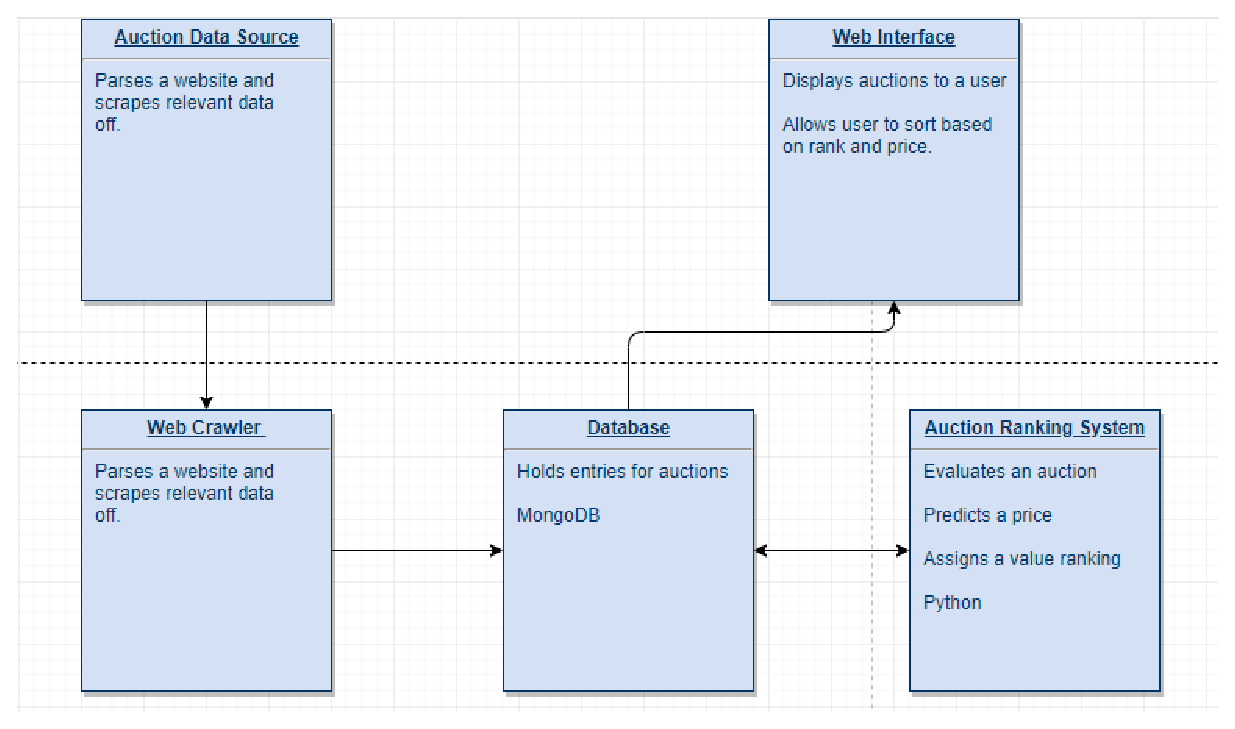
\includegraphics[scale=0.75]{flow_capture}
\caption{Flow Design}
\label{fig:flow}
\end{figure}


\section{Progress}  % screenshots here
Our Auction Hunter program currently scrapes entries from IAAI, stores them in a database, performs value calculations, and displays to a user through a web interface. 

To perform the web scraping, we are using the 'Scrapy' tool, which interfaces directly with our our database. We simply had to modify a pipeline to send the auction entries to mongoDB instead of saving to a file. To perform the value calculation, we use the mileage and damage information to skew the value of the car in one direction or another. This is a naive implementation that will need to be improved and tested. One of the biggest precursors to improving the value estimation is data availability. We are currently hosting our database on a personal server, which means we can all access the database from home. To make viewing the contents of the database easier, we are using mongoDB's GUI, called 'compass'. Below is a screenshot of our current database entries. \cite{MongoDB}

\begin{figure}[H]
\centering
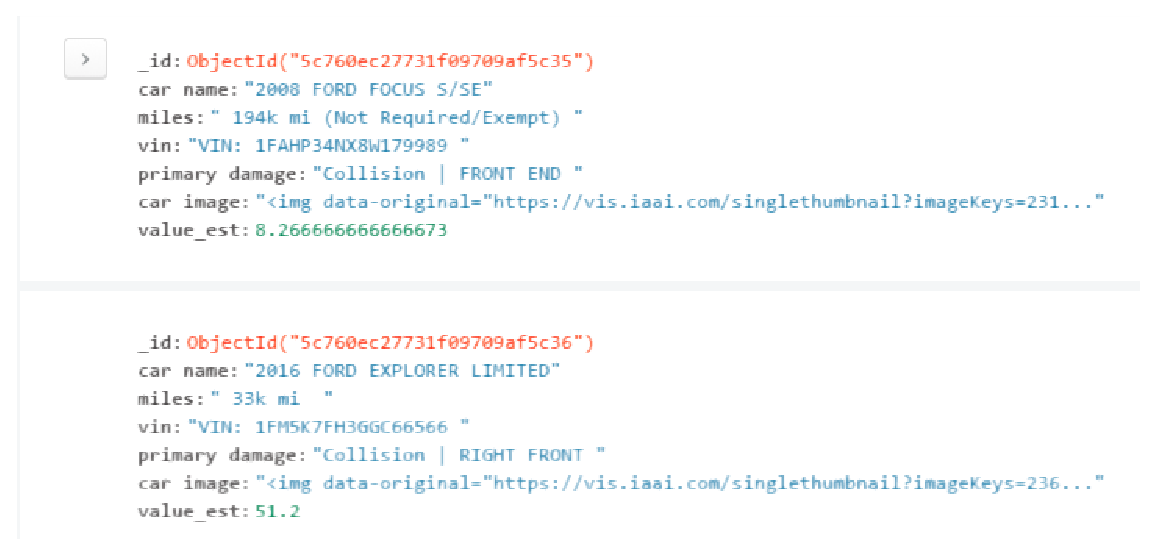
\includegraphics[scale=0.85]{db}
\caption{Database entries}
\label{fig:mongoDB}
\end{figure}

\subsection{Web Interface Progress}
Auction Hunter's web site is comprised of two main parts: the frontend and the backend. The backend is hosted on the server and serves the frontend to the visitor. The frontend is downloaded onto their computer and then run in their web browser. The frontend then makes REST API calls to the backend to interact with the database. REST is a widely used API architecture that defines and formalizes the interaction between two systems. 
The frontend uses the REST API to makes various types of calls including logging in a user, updating settings, requesting auction data, etc. The backend is written in Python using a library called Django. Using Django, Auction Hunter can handle logins, modify the database, and send emails and other notifications. The frontend is written in JavaScript using the React framework to generate the layout and user interaction with the server. Users of Auction Hunter will only ever interact directly with the frontend, which then will translate the necessary actions into REST commands to send to the server. 

\begin{figure}[H]
\centering
\includegraphics[scale=0.4]{HomePage.eps}
\caption{HomePage of Auction Hunter}
\label{fig:homepage}
\end{figure}

Shown above is the front page to our website. It shows the six most recent cars added to the database along with some basic details about the cars. You can then click on the car and brings you to a more detailed page about the auction its self. There is also a search bar that does a basic keyword search on the car. 

% Yufei: something pseudocode for web scrawler in Python
\subsection{Web Scraper Progress}
When customers are trying to buy a salvage car and they will want to see the prices at different platforms at a single place. In such situations, Web crawler will full play its function on building an aggregator platform.

IAAI.com is a website that sells salvage cars.\cite{IAAI} It will be our test site, and we are going to scrape Timed Auctions for salvage cars. The first step is to generate a basic spider using python:

\begin{minted}{python}
scrapy crawl iaaibot

\end{minted}

That is what the IAAI Timed Auctions page looks like:

\begin{figure}[H]
\centering
%\includegraphics[scale=0.5]{AuctionSearchResults}
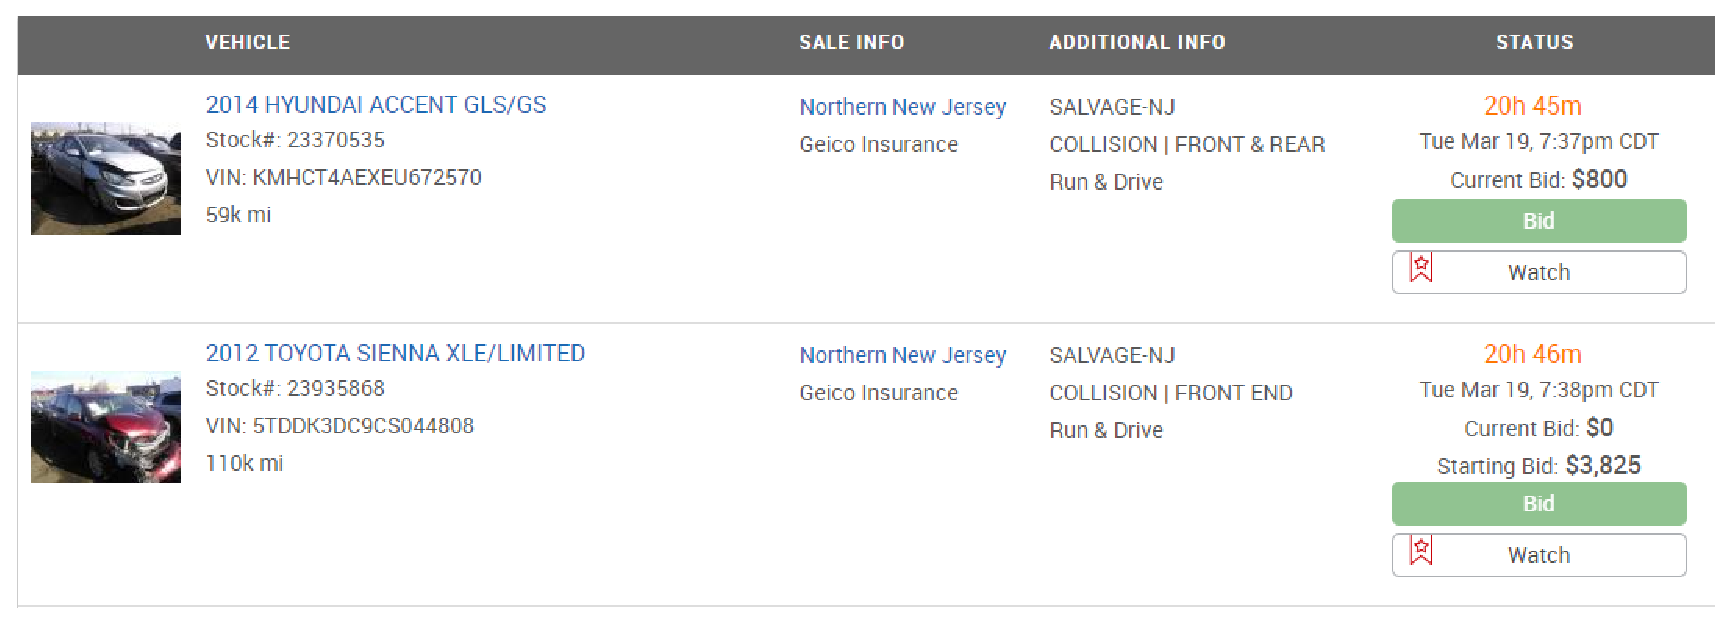
\includegraphics[scale=0.5]{timed_auction}
\caption{Timed Auctions Page}
\label{fig:auction}
\end{figure}

From this page, the following data about a salvage car needs to be extracted:

\begin{itemize}
\item Salvage car name
\item Salvage car miles
\item Salvage car vin
\item Salvage car primary damage
\item Salvage car image's url
\end{itemize}

\textbf{Extracting the URLs include salvage car photo:}

After searching through the web page source code by using the developer tools of Chrome and Google extension SelectorGadget. We found that the car photos are stored under vis.iaai.com with "imageKeys" and their CSS labels are ".lazy".

%\begin{figure}[ht]
%\centering
%\includegraphics[scale=0.55]{salvagecarphoto}
%\caption{Salvage Car Photo}
%\label{fig:salvage}
%\end{figure}

%\begin{figure}[ht]
%\centering
%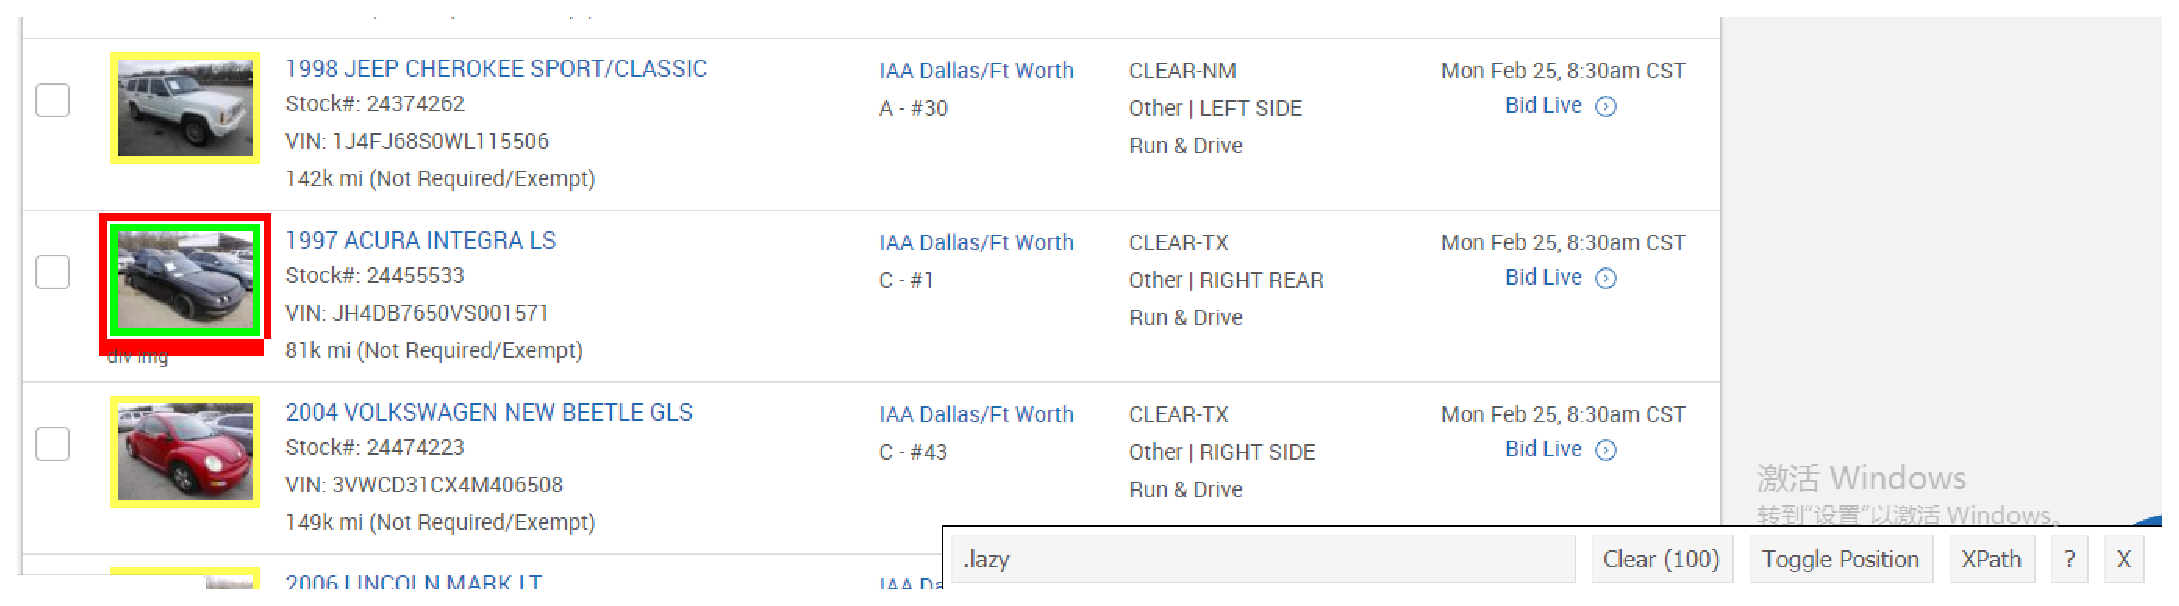
\includegraphics[scale=0.55]{SelectorGadgetTech}
%\caption{SelectorGadget Tech}
%\label{fig:salvage2}
%\end{figure}

The CSS labels ".lazy" can be used to extract image URLs. 
\begin{minted}{python}
CarImage = response.css('.lazy').getall()
\end{minted}
\textbf{Extracting the URLs include salvage car Vin:}

We can use a similar method to find VIN's location which is an attribute of the \textless a~ p:nth-child(3)\textgreater  tag.

\begin{figure}[H]
\centering
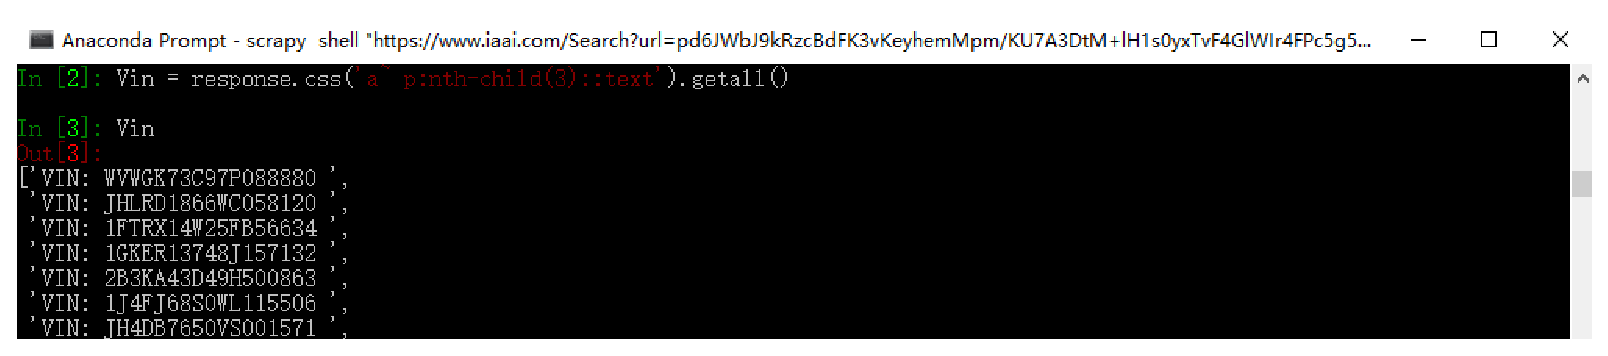
\includegraphics[scale=0.65]{vinscrape}
\caption{Scraping Vin}
\label{fig:vin}
\end{figure}

%\centerline{
% 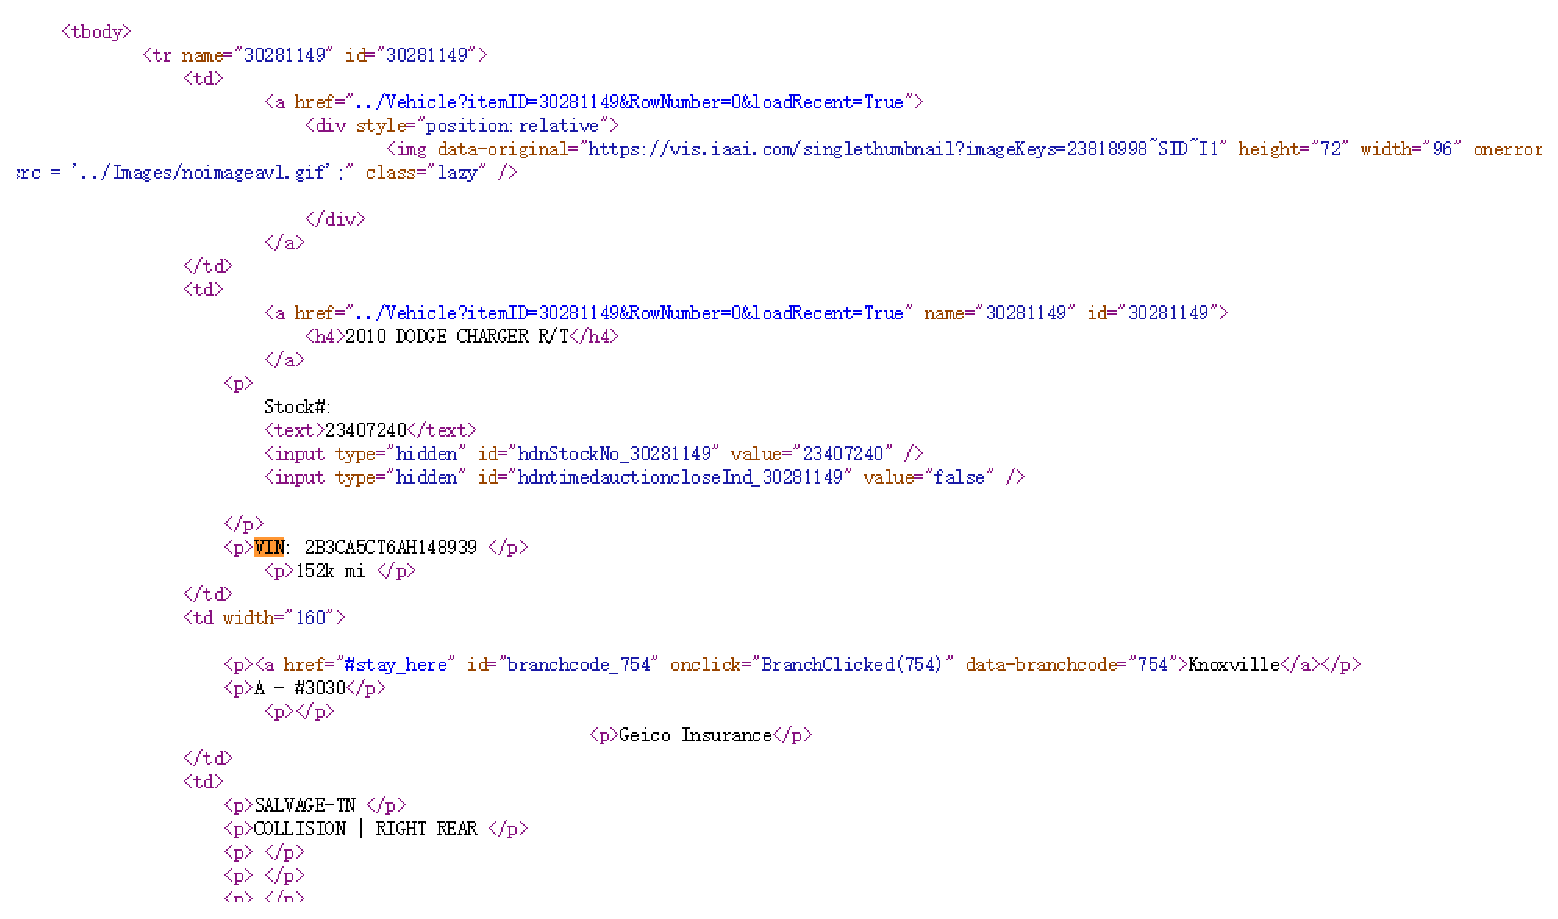
\includegraphics[width=80mm]{salvagecarvin}
% }

\begin{minted}{python}
Vin = response.css('a~ p:nth-child(3)::text').getall()
\end{minted}

\textbf{Extracting the URLs include salvage car name, miles, and primary damage:}

Similarly, we are able to extract the name, miles and primary damage or any other necessary data of salvage car.
\begin{minted}{python}
#Extracting the content using css selectors
Vin = response.css('a~ p:nth-child(3)::text').getall()

\end{minted}

\textbf{Time to download the extracted photos of salvage car:}

As mentioned in Design Document, Scrapy provides the images pipelines: once we got the data from website, we are able to pass them through different pipelines. By taking advantage of this function, the image pipeline allows us to download extracted photos of salvage car. In addition, we are able to convert the format of images and generate thumbnail.

\begin{minted}{python}
#enable the images pipeline.
SalvageCarPhotos_PIPELINES='scrapy.pipelines.images.ImagesPipeline': 1
#set the local download address.
Photo_Store = 'Users/Desktop/SalvageCarPhotos/'
\end{minted}

\begin{minted}{python}
#Generate two kinds of thumbnail for each salvage car photo, one small, one large.
GenerateThumbnail = {'small': (20, 20), 'large': (100, 100),}

\end{minted}


\section{Future Plans}
\subsection{Web Interface Advancements}
\begin{itemize}
    \item Once database has more data scrapped from auction site, display more in detail page.
    \item Make logging in easier by displaying better errors when the username or password is incorrect.
    \item Finish allowing the user to set and recieve alerts about auctions.
\end{itemize}

\subsection{Database Advancements}
\begin{itemize}
    \item Database will need to be expanded to hold more elements, and more attributes from each element. 
    \item Value estimations will need to take into account the additional elements. 
    \item Value estimations will have to be studied and tested more thoroughly. This will include creating trend visualizations, and compare to the current bid price to find where it overvalues/undervalues auctions. 
    
\end{itemize}

\subsection{Web Crawler Advancements}

\begin{itemize}
\item Instead of just scraping the stuff from the current page, we want quotes from all the pages in the website. The corresponding solution might be that we could get the anchor element like "next" or "next page" to set a for loop to keep the crawling going through all the pages on IAAI. 
\item We only have extracted the url of car images rather than the exact images. We are looking for a method to download the extracted photos of salvage car to local. The corresponding solution includes using the images pipeline in Scrapy.
\item We are working on consolidating the extracted data of salvage car into our database. The corresponding solution is that we need to extract data with a better logic. For example, removing all redundancies. 

\end{itemize}

\section{Problems}
One issues that we are running into is the difficulty in updating our database in real time to match the original source. New auctions are created and removed every day, and our database will have to reflect that in order to stay relevant. Our current implementation doesn't allow for routine updates, meaning our database can become out of sync quickly. 

Another problem faced along the way was implementing features that other components cannot use effectively. This happened when a handful of database features were implemented for adding and reading entries. We later found out that our web scraper was able to interface with the database automatically, completely bypassing the work that was completed on the database. Although this is a much easier solution, it resulted in some wasted implementation time. This may have been something that could have been avoided if more research was done into how each component will work together before implementation started. One benefit was that initially going about this the hard way made it easier to implement future database advancements, where existing code could be salvaged. 


\section{Code Snippets}
\subsection{Web Scraper}
The following snippet demonstrates how the web scraper communicates with the database, which is called the "mongoDB pipeline". 

\begin{figure}[H]
\centering
\begin{minted}{python}
    def open_spider(self, spider):
        self.client = pymongo.MongoClient(self.mongo_uri)
        self.db = self.client[self.mongo_db]

    def process_item(self, item, spider):
        self.db[self.collection_name].insert_one(dict(item))
        return item
\end{minted}
\caption{Calculate value estimation}
\end{figure}
Scrapy will call open\_spider before it begins scraping, which establishes its connection to the mongo database. Whenever it processes an item, it inserts that item into the database. 

\subsection{Database and Value Calculation}
The below code snippet is how value calculations are added to all the available entries in the database. It may seem logical to instead calculate these values when the database is first populated. However, Scrapy makes it very easy to insert directly into the database, so it is easier to populate automatically, then sanitize and enhance the database later on. 
\begin{figure}[H]
\centering
\begin{minted}{python}
    #return a cursor object of all entries with a certain year. 
    result_cursor = db.collection.find( { year: { "gt:" int(year) } } )
    #Find the total number returned 
    count = result_cursor.collection.count_documents({})
    #Parse through all returned entries
    for x in range(count):
        #Go to the next (this will point to the first entry after the first call)
        current_entry = result_cursor.next()
        #Get value estimation number
        value = enhancer.getValueEstimation(current_entry)
        currentVin = current_entry.get("vin")
        #Add the value estimation to the database as a new attribute
        database.scrapy_items.update_one({"vin": currentVin}, {"\$set": {"value_est": value}})
\end{minted}
\caption{Adding value calculation to database}
\end{figure}

The current value estimation is very simplistic. This is chosen more as a initial best guess, and will be improved as more data is available. Currently, the value estimation is only based on the damage and miles. The 'damage' variable is calculated based on the severity of the damage description. This ranges from 0-5. These values are weighted, by 'milesWeight' and 'damageWeight' which both affect how much that calculation changes the value. These configuration variables are defined before any estimation is performed. 

\begin{figure}[H]
\centering
\begin{minted}{python}
    #Miles in thousands
    value -= ((miles*2)/150.0 - 1)*self.milesWeight
    #Damage from 0 to 5(most impactful damage) 
    value -= damage*(self.damageWeight/2.0)
\end{minted}
\caption{Calculate value estimation}
\end{figure}

\subsection{Web Interface}
The most important part of the web interface is the displaying of data from the database. The code below shows how a single row from the database represents a car and then that car's data is then displayed nicely to the user, using HTML and CSS. The return function has to return all of the cars the home page needs to display. We created an inline function to create a single auction card which is a library we created to display a single auction to the user. The map function takes each car in a list and returns a list of HTML formatted code that is then returned to the main function to display. 

\begin{figure}[H]
\begin{minted}{html}
return ( 
  <div><Grid container spacing={24}>
    {this.cars.map((car) => {
      return ( <Grid item xs={6}>
                 <AuctionCard
                   carImage={car.carImage}
                   carName={car.carName}
                   miles={car.miles}
                   vin={car.vin}
                   damage={car.damage}
                 />
               </Grid>
             )
         })} </Grid></div>); })
\end{minted}
\caption{web}
\end{figure}


\bibliographystyle{IEEEtran}
\bibliography{IEEEabrv,bib}


\end{document}
